\question (北京航空航天大学,2003年)已知带权连通无向图G=(V,E),其中V=\{v1,v2,v3,v4,v5,v6,v7\},E=\{(v1,v2)10,(v1,v3)2,(v3,v4)2,(v3,v6)11,(v2,v5)1,(v4,v5)4,(v4,v6)6,(v5,v7)7,(v6,v7)3\}(注:顶点偶对右下角的数据表示边上的权值),则从源点v1到顶点v7的最短路径上经过的顶点序列是(
)
\par\twoch{v1,v2,v5,v7}{\textcolor{red}{v1,v3,v4,v6,v7}}{v1,v3,v4,v5,v7}{v1,v2,v5,v4,v6,v7}
\begin{solution}由于是选择题,因此最简单的方法不需要画图,直接算出四条路径的距离,取最小者。可知A、B、C和D的路径长度分别为18、13、15和24。因此本题选B。
\end{solution}
\question (中南大学,2005年)求最短路径的floyd算法的时间复杂度为( )
\par\twoch{O(n)}{O(n+e)}{}{\textcolor{red}{}}
\begin{solution}考察floyd算法的时间复杂度。floyd算法是求图中所有点对的最短路径,它的时间复杂度为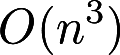
\includegraphics[width=0.43750in,height=0.19792in]{texmath/6054ee5Cdpi7B3507DO28n5E329}
\end{solution}
